\documentclass[times, 10pt,dvipdfmx]{jsarticle}
\usepackage{graphicx}  
\usepackage{times}
\usepackage[most]{tcolorbox}
\usepackage{ascmac}
\usepackage{amsmath}
\usepackage{fancybox} 
\usepackage{version}
\usepackage{mdframed}
\usepackage{url}
\usepackage{xcolor}
%\usepackage{chapterbib}
\usepackage{tboxit}
\usepackage{boxedminipage}
\usepackage{rdbkbox}
\usepackage{bm}
\makeatletter
\renewcommand{\figurename}{Figure}
\renewcommand{\tablename}{Table}
\renewcommand{\refname}{References}
\def\theequation{\thesection.\arabic{equation}}
\def\thefigure{\thesection.\arabic{figure}}
\def\thetable{\thesection.\arabic{table}}
\@addtoreset{equation}{section}
\@addtoreset{figure}{section}
\@addtoreset{table}{section}
\makeatother 
\setlength{\oddsidemargin}{0mm}
\setlength{\evensidemargin}{0mm}
\setlength{\textwidth}{16cm}
\newtheorem{kadai}{Exercise}[section]
\newtheorem{tisiki}{Advanced}[section]
\newtheorem{reidai}{Example}[section]
\newenvironment{kaisetsu}
{\vspace{5mm}\begin{center}\dotfill Explanation \dotfill\end{center}}
{\begin{center}\dotfill EoE \dotfill\end{center}\vspace{5mm}}
\newenvironment{theorem}%
{\begin{mdframed}[backgroundcolor=lightgray,linewidth=0]}%
{\end{mdframed}}
\newenvironment{advanced} 
{\vspace{5mm}\begin{center}\Dotfill \\
\Dotfill Advanced Study \Dotfill\end{center}}
{\begin{center}\Dotfill End of Advanced Study \Dotfill \\
\Dotfill 
\end{center}\vspace{5mm}}
\definecolor{Gray}{gray}{0.85}
\excludeversion{kaisetsu}
\tcbset{
    frame code={}
    center title,
    left=0pt,
    right=0pt,
    top=0pt,
    bottom=0pt,
    colback=gray!70,
    colframe=white,
    width=\dimexpr\textwidth\relax,
    enlarge left by=0mm,
    boxsep=5pt,
    arc=0pt,outer arc=0pt,
    }
%
%
%
%
\DeclareMathOperator*{\argmax}{argmax}
\newcommand{\figSize}{0.7}
\newcommand{\hhline}{\begin{center}\begin{tabular}{c}\hline\hline\end{tabular}\end{center}}
\newcommand{\ffbox}[1]{\centerline{\vspace{1cm}\fbox{\parbox{0.8\textwidth}{#1}}\vspace{1cm}}}
%\newcommand{\ffbox}[1]{{\vspace{1cm}\fbox{\parbox{1.0\textwidth}{#1}}\vspace{1cm}}}
\newcommand{\ftbox}[2]{\vspace{5mm}\tboxit{#1}{\vbox{\hsize 0.8\textwidth #2}}}
%\newcommand{\bm}[1]{\boldmath{#1}}
%\renewcommand{\dotfill}{\vspace{10mm}\dotfill}
\setlength{\textheight}{630pt}
\newcommand{\obox}[1]{\vspace{5mm}\ovalbox{#1}}
\newcommand{\vs}{\vspace{5mm}}
\newcommand{\dia}{\vspace{3cm}\centering{$\diamond$ \hspace{1cm} $\diamond$ \hspace{1cm} $\diamond$}\vspace{3cm}}
\usepackage{fancybox}
\newtheorem{prog}{program}[section]
\newenvironment{program}
{
  \VerbatimEnvironment
  \baselineskip=.40\normalbaselineskip
  \begin{Verbatim}
}
{
  \end{Verbatim}
  \baselineskip=\normalbaselineskip
  \noindent
}
%%\newcommand{\na}{\begin{quote}\setlength{\baselineskip}{12pt}\begin{verbatim}}
%\newcommand{\ea}{\end{verbatim}\end{equote}}
%\newenvironment{FRAME}{\begin{trivlist}{\item[]
%\hrule
%\hbox to \linewidth\bgroup
% \advance\linewidth by -30pt
% \hsize=\linewidth
% \vrule\hfill
% \vbox\bgroup
% \vskip15pt
%  \def\thempfootnote{\arabic{\mpfootnote}}%
%  \begin{minipage}{\linewidth}}{%
%\end{minipage}\vskip15pt
%\egroup\hfill\vrule
%\egroup\hrule
%\end{trivlist}}

\pagestyle{plain}
\begin{document}
\title{DS1　微分・積分で何ができるか}
\date{2025年4月14日}
\author{三次　仁}
\maketitle
この授業では、データサイエンスの実践のため＋数学的思考を身に着けるために微分・積分を学ぶ。授業は共通教材と、参考書\cite{tazawa}に沿って進める。どちらも微積分の前提知識として数、集合、関数が順序だてて構成されている。積分を学ぶためには微分が必要で、微分を知るには、極限を理解する必要があり、その前には関数や集合の知識が必要であるのはその通りなのだが、多くの場合、データサイエンスの「実践」が目的である我々にとっては、まず具体的に微積分がなぜ必要なのか、微積分を学ぶことで何ができるようになるのか、を理解することも重要と思う。少し正確性は失っていたとしても、微分積分が我々が扱う現実の問題にどのように役立つのか見通しがつけば、抽象的になりがちな数学や理論を頑張る気力も維持しやすいはずだ。

\vspace{5mm}
このノートでは具体的な問題を例示しながら、なぜ微分・偏微分・積分が重要なのか、主としてエンジニアの視点と経験から説明を試みる。

\section{微分}
\subsection{データの傾向を調べる(回帰分析)}
微分(differential、微分計算の結果はderivative)は、様々な最適化の基本である。例えばある地域の家賃$y$万円と、部屋の広さ$x$~$\mathrm{m^2}$のデータを集めて、相場を推定する仕事を担当したとしよう。$i$番目の家賃と、部屋の広さのデータを$y_i, x_i$で表して、データがTable~\ref{tab:renttab}のように$15$個集められたとする。
\begin{table}[hbt]
\centering 
\caption{部屋の広さと家賃に関するデータ}
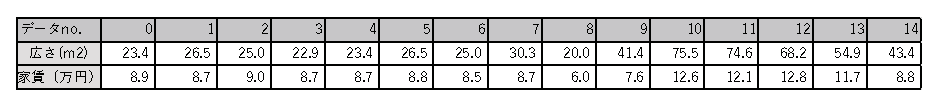
\includegraphics{renttab.eps}
\label{tab:renttab}
\end{table}
このデータを散布図で表すとFig.~\ref{fig:rent}である。
\begin{figure}[hbt]
\centering
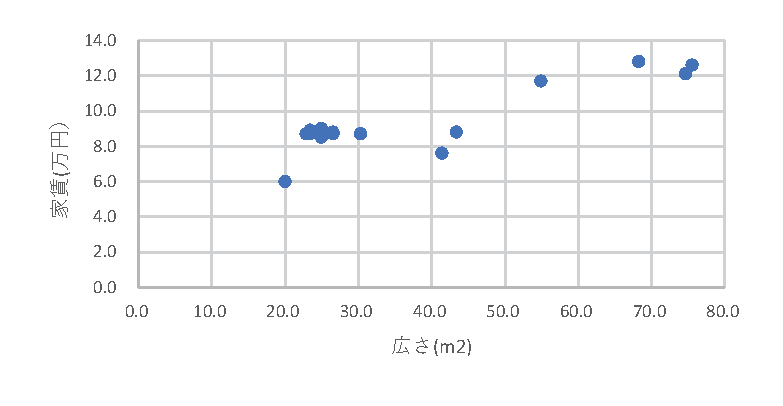
\includegraphics{rent.eps}
\caption{部屋の広さと家賃のデータ}
\label{fig:rent}
\end{figure}

\subsubsection{相場を一つの変数を用いて表す場合}
少し乱暴だが、部屋の広さ$x$を与えると家賃相場$y$が
\begin{equation}
y = a x 
\label{eq:regsimple}
\end{equation}
で与えられるとする。変数$a$を適切(この場合0.2ぐらい）に選ぶと集めたデータの傾向に近似した直線が引ける(Fig.~\ref{fig:reg}). このようにデータの関係を明らかにすることは回帰分析（regression analysis)と呼ばれる。
\begin{figure}[hbt]
\centering
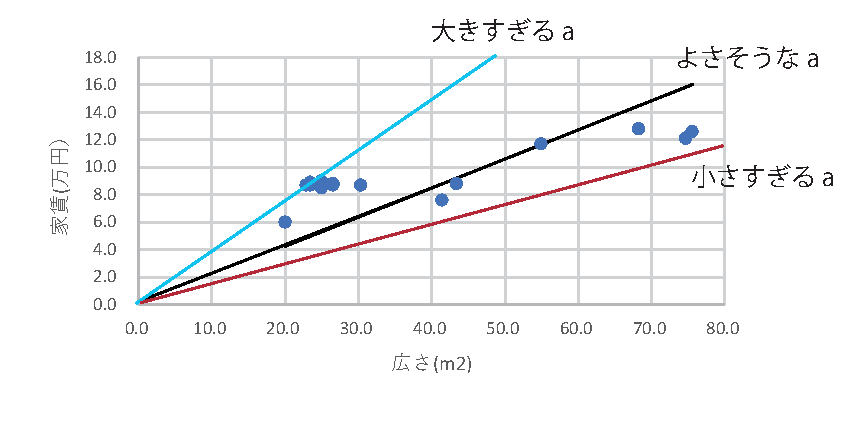
\includegraphics{reg.eps}
\caption{部屋の広さと家賃のデータを様々な$a$で近似}
\label{fig:reg}
\end{figure}
データから目視あるいは試行錯誤で$a$を決めることは、厳密でなくてよいなら簡単である。同様に、Fig.~\ref{fig:reg}の小さすぎる$a$や、大きすぎる$a$の直線が、データをうまく近似していないことも直観で明らかである。


ある$a$がよさそうとか、よくないは、データを表す点群（マーカー群）に対して、求めた直線$y=ax$が上下バランスよく貫いているかどうかで判断できる。この「バランスの良さ」は$a$を変数とする数式（関数:function)$f(a)$で計算できるとしよう。$f(a)$は損失関数(loss function)と呼ばれる。

$a$に何かの値を仮に入れた場合、各データ点について式\ref{eq:regsimple}を用いて$ax_i$で計算した値と、観測した$y_i$は多くの場合、一致せず誤差$e_i$が発生する。式で書けば以下である。
\begin{equation}
e_i = y_i - a x_i
\end{equation}

$a$が大きすぎたり小さすぎたりすれば、誤差も増える。この誤差はプラスマイナスどちらにもなる可能性があるので、$a$が適切でない場合には損失関数がプラスに増えるように、それぞれの誤差の二乗を総和した数を損失関数として用いることが良く行われる。誤差がプラスであってもマイナスであっても二乗すれば必ずプラスの値になるためである。このとき、損失関数$f(a)$はEq.~\ref{eq:loss}で与えられる。
\begin{equation}
f(a) = (y_o - a x_o)^2 + (y_1 - ax_1)^2 + \cdots + (y_{14} - a x_{14})^2
\label{eq:loss}
\end{equation}

$a$の値を0から1.0まで0.1刻みで変化させて損失関数を計算するとFig.~\ref{fig:loss}のようになる。

\begin{figure}[hbt]
\centering
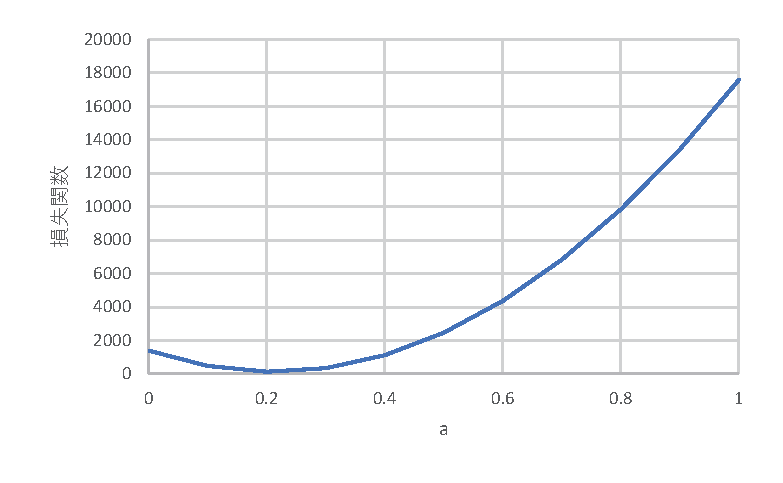
\includegraphics{loss.eps}
\caption{係数$a$を変化させた場合の損失関数$f(a)$の値の変化}
\label{fig:loss}
\end{figure}
Fig.~\ref{fig:loss}を見ると、$f(a)$は滑らかに変化し、$a=0.2$くらいで一番小さくなることがわかる。$a$が微小な量$\Delta a$変化したときの$f(a)$の変化の割合を傾き(tilt)と呼ぶ（Fig.~\ref{fig:tilt})。
\begin{figure}[hbt]
\centering
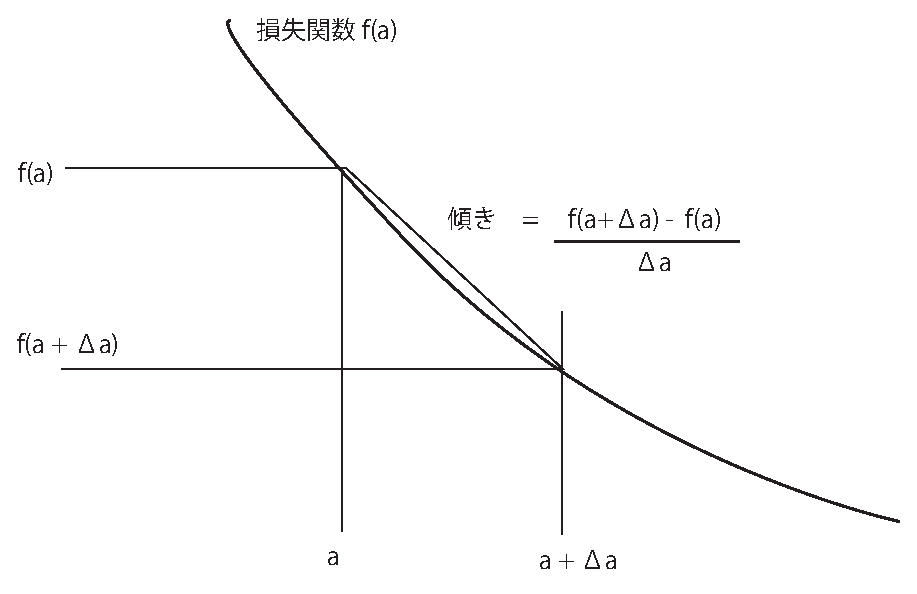
\includegraphics[width=\figSize\textwidth]{tilt.eps}
\caption{ある点a近くでの損失関数の傾き(微分）}
\label{fig:tilt}
\end{figure}
一番小さい損失関数を与える$a$では、傾きはゼロとなる。この点の近くで少し$a$が変化しても、ほとんど$f(a)$の値は変わらないとも解釈できる。この傾き=$f(a)$が$a$に関する微分$\frac{df}{da}$であり、{部屋の広さと家賃の相場をデータから求めることは、$f(a)$の微分$\frac{df}{da}$がゼロとなる$a$を求めることと等価である。}

Eq.~\ref{eq:loss}を$a$に関して微分して、それがゼロになることを式で表せば以下となる。どうやって微分が行われたか理解できなくても今は問題ない。
\begin{equation}
\frac{df}{da} = 2(y_o - ax_o) (-x_o) + 2(y_1 -ax_1)(-x_1) + \cdots + 2(y_{14} - a x_{14}) (-x_{14}) = 0 
\label{eq:diffloss}
\end{equation}
Eq.~\ref{eq:diffloss}の$a$以外の数はすべて既知なので、次のようにまとめることができる。
\begin{equation}
(x_o^2 + x_1^2 + \cdots + x_{14}^2) a = (x_o y_o + x_1 y_1 + \cdots + x_{14} y_{14})
\end{equation}
したがって$a$は観測したデータだけを用いて
\begin{equation}
a = \frac{x_o y_o + x_1 y_1 + \cdots + x_{14} y_{14}}{x_o^2 + x_1^2 + \cdots + x_{14}^2}
\end{equation}
と計算することができる。観測データの数字を入れて計算すると、$a=0.212$が得られ、このときの損失関数は126.1である。微分を使えばFig.~\ref{fig:rent}のデータを用いてFig.~\ref{fig:reg}の「よさそうな$a$」を直接求められるのだ。
\vs

ここで説明した誤差関数として誤差の二乗を用い、損失関数を最小化する変数を求める方法は最小二乗法(Least square methodあるいはMinimum mean squared error (MMSE))と呼ばれ、良く用いられている。しかし、観測エラーや、入力間違いなどで生じる外れ値(outlier)に過度に敏感に反応する(過剰適合：overfitting)する傾向があることも知られており、それを解決する方法として、さまざまな正則化方法(regularization)が提案され、使われている。このあたりは統計の授業で学ぶ（はず）。



\subsubsection{変数が２つある場合}
部屋がいくら狭くても、家賃はゼロにはならないので、相場を表す式を傾き(tilt)$a$と、切片(section) $b$を使って以下で
\begin{equation}
y = a x + b
\label{eq:souba}
\end{equation}
表すことを考える。

この場合、最小二乗法による損失関数は$f(a, b)$と２つの変数で表現され、
\begin{equation}
f(a,b) = (y_o - a x_o-b)^2 + (y_1 - ax_1 - b)^2 + \cdots + (y_{14} - a x_{14} -b)^2
\label{eq:loss2}
\end{equation}
となる。$a,b$が変わると損失関数の値が変わるので、もっとも小さい損失関数を与える$a,b$により、Eq.~\ref{eq:souba}の形で家賃相場を求めることができる。前の式(Eq.~\ref{eq:loss})では変数は$a$のみ、今回は$a,b$の２つを調整できるので、より損失関数の小さい家賃相場を得ることができるはずである。本当はそういう形にはならないのだが、イメージとしてはFig.~\ref{fig:loss2}のように$a,b$平面に対して立体的に損失関数が計算できる。
\begin{figure}[hbt]
\centering
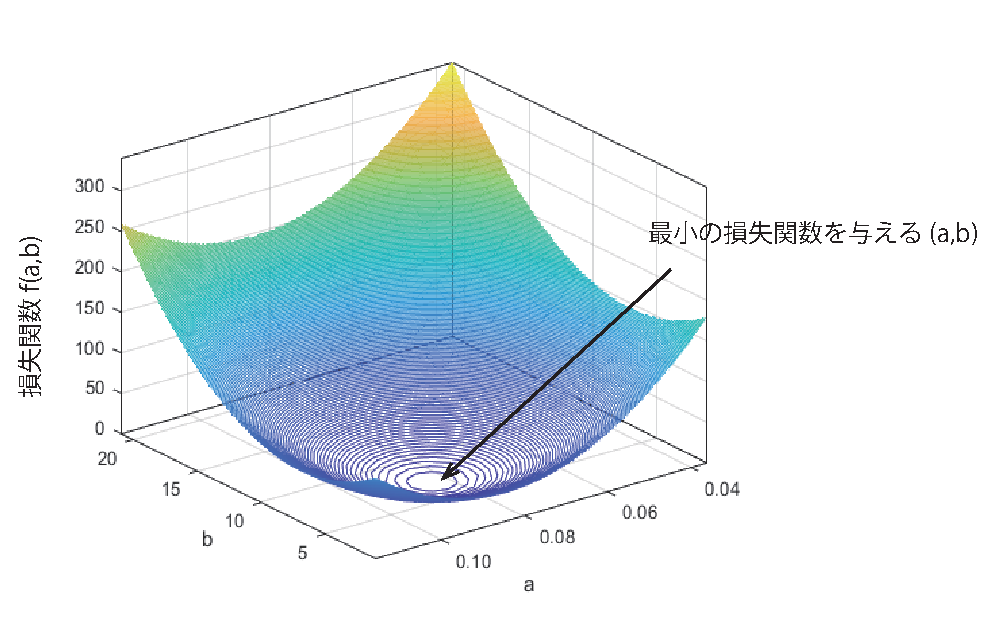
\includegraphics{loss2.eps}
\caption{相場係数$a, b$を変化させた場合の損失関数$f(a, b)$の値の変化のイメージ}
\label{fig:loss2}
\end{figure}

この損失関数において、$b$を一定値と想定して、$a$で微分することを偏微分(partial differential)と呼び、$\frac{\partial f}{\partial a}$で表す。Fig.~\ref{fig:loss2}で$a$軸の方向の損失関数の傾きを計算しているのである。最小の損失関数を与える$a,b$の点において、$a$方向の傾きはゼロとなるはずである。
\begin{equation}
\frac{\partial f}{\partial a} = 2(y_o-ax_o - b)(-x_o) + 2(y_1 - ax_1 - b) (-x_1 ) + \cdots + (y_{14}-a x_{14} -b) (-x_{14}) = 0
\end{equation}
同様に$a$を一定値と想定して$b$で損失関数を偏微分すると$b$方向の傾きを求めることができ
\begin{equation}
\frac{\partial f}{\partial b} = 2(y_o-ax_o - b)(-1) + 2(y_1 - ax_1 - b) (-1 ) + \cdots + (y_{14}-a x_{14} -b) (-1) = 0
\end{equation}
これも、最小の損失関数を与える$a,b$点でゼロになる。このように偏微分を用いることにより、１つの損失関数から変数と同じ数だけの等式（連立方程式）を導くことができる。

これら二式で未知の変数は$a,b$のみで他は既知であることから、まとめて書くと
\begin{eqnarray}
(x_o^2 + x_1^2 + \cdots + x_{14}^2 ) a + (x_o + x_1 + \cdots + x_{14}) b &=& (x_o y_o + x_1 y_1 + \cdots + x_{14}y_{14}) \nonumber \\
 (x_o + x_1 + \cdots + x_{14}) a + 15 b &=& (y_o + y_1 + \cdots + y_{14}) 
\end{eqnarray}
となり\footnote{式中の15はデータの数である}、これは連立方程式の一般的な形であり、
\begin{equation}
\left[\begin{array}{cc}
(x_o^2 + x_1^2 + \cdots + x_{14}^2 ) & (x_o + x_1 + \cdots + x_{14})  \\
 (x_o + x_1 + \cdots + x_{14})  & 15 
 \end{array}\right]
 \left\{\begin{array}{c} a \\ b \end{array}\right\} = 
 \left\{\begin{array}{c} (x_o y_o + x_1 y_1 + \cdots + x_{14}y_{14}) \\  (y_o + y_1 + \cdots + y_{14}) 
 \end{array}\right\}
 \end{equation}
線形代数で学ぶ逆行列を使って次のように解くことができる。
\begin{equation}
 \left\{\begin{array}{c} a \\ b \end{array}\right\} = \left[\begin{array}{cc}
(x_o^2 + x_1^2 + \cdots + x_{14}^2 ) & (x_o + x_1 + \cdots + x_{14})  \\
 (x_o + x_1 + \cdots + x_{14})  & 15 
 \end{array}\right]^{-1}
 \left\{\begin{array}{c} (x_o y_o + x_1 y_1 + \cdots + x_{14}y_{14}) \\  (y_o + y_1 + \cdots + y_{14}) 
 \end{array}\right\}
 \end{equation}
この計算をすると$a=0.085$, $b=6.150$となり, 最小の損失関数$f(a,b)=11.44$となって、$a$のみを用いた場合より、正確に相場を近似できる（Fig.~\ref{fig:reg2})。
\begin{figure}[hbt]
\centering
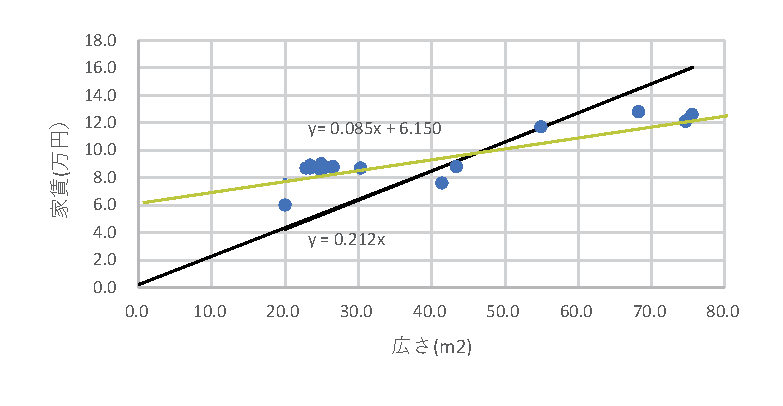
\includegraphics{reg2.eps}
\caption{一変数と二変数による回帰分析の違い}
\label{fig:reg2}
\end{figure}

\vs

こうした回帰分析機能は、Rなど統計処理のソフトウェアや、python pandas, エクセルなどにも組み込まれており、簡単な問題であれば自分で微分したり、プログラムを作成する必要はない。
しかし学習や研究が進むと、損失関数を問題に合わせて定式化し、最適化するため自ら数式を微分することはしばしば起こる。微分や偏微分を理解していれば、自分で実際にやらないにしても、問題解決に貢献できるかもしれない。逆にツールに依存してしまうと、ツールの想定と少しでも外れた問題に対応できない。例えば先述の外れ値処理などが典型的である。
\vs

多くの変数候補があり、変数と損失関数の関係の数式化ができない場合でも、機械学習を用いることで徐々に損失関数を最適化する変数を求めることが近年急速に発展している。機械学習の多くは、画像や音声などの対象データを、二以上に分類する分類問題(classification)に帰結できる。この際、分類に用いる損失関数（損失関数が大きいと分類Ａ、小さいと分類Ｂなど）と対象データに含まれる多くの変数の関係が確立されていなくとも、損失関数の近似的な微分（勾配）を用いて、変数の貢献度を表す重みを少しづつ調整できる。先ほどの$a,b$も変数$x$に対する重みである\footnote{$b$は直接変数ではないが、モデル化するための定数であり、重みとして扱うことができる}。


\section{微分方程式と積分}
ここまで回帰分析を例にとって最適化における微分の有効性を説明したが、微分は、この他にもエンジニアリングや経済の分野で、事象や運動を微分を含む方程式（微分方程式）で表すことに活用されている。

たとえば時間$t$で位置$x$が変わる物体があるとして、ある短い時間$\Delta t$に$\Delta x$だけ移動したとすると時間$t$における速度$v$は
\begin{equation}
v = \frac{\Delta x}{\Delta t}
\end{equation}
であり、この$\Delta t$を限りなくゼロに近づけた時に収束する値が$x$の時間微分$\frac{dx}{dt}$である。つまり位置の時間微分は速度である。
さらに速度の時間微分（位置の二階微分)$\frac{dv}{dt} = \frac{d^2x}{dt^2}$は加速度である。加速度に質量$m$を掛けると与える力$F$と等しいとするニュートンの運動方程式はよく知られている。
\begin{equation}
m\frac{d^2x}{dt^2} = F
\label{eq:newton}
\end{equation} 
こうした微分方程式は、電磁気学のマックスウェル方程式、流体力学のナビエストークス方程式、経済学のブラックショールズ方程式、
、量子力学のシュレディンガー方程式など、多くの事象の時間的・空間的変化の原理を説明している。つまりこれらの方程式を厳密に解ければ、運動や株価、天気の時間変化を「すべて正確に予測すること」ができる。

上の運動の問題であれば、時間に応じた力の変化$F(t)$が既知であれば、物体の時間に応じた位置$x(t)$は式\ref{eq:newton}を積分することで求められる。積分操作が今の段階でわからなくてもよいが、加速度を時間積分すると速度が得られ、速度を時間積分すると位置が得られる。運動方程式を積分すれば、天体運動もロケットの軌道も予想できるのである。

\begin{eqnarray}
\frac{dx}{dt} &=& \int_0^t F/m dt \\
x &=& \int_0^T \int_0^s F/m dt ds
\end{eqnarray}

中学や高校で扱ってきた方程式は微分項を含まない代数方程式(algebraic equation)である。上の式で$F/m$が時間に関わらず一定値であれば
時間で変化する$x$を次のように予測できる。$C_1$, $C_2$は積分定数と呼ばれる定数である。

\begin{eqnarray}
\frac{dx}{dt} &=& \int_0^t F/m dt = F/m t + C_1 \\
x &=& \int_0^t \int_0^t F/m t  dt = \frac{1}{2} F/m t^2  + C_1t + C_0
\end{eqnarray}

\vspace{5mm}
特別な問題を除けば、$F$が時間で変化する場合に、式の形で積分を表すことができない（定積分）。コンピュータを使って積分の近似値を求める手法（シミュレーション:simulation)が様々開発され、利用されている。


天気予報での雨雲の動きの予想や、飛沫飛散などのシミュレーションでは、本来時間的に連続している変数（たとえば位置$x$)を短い時間刻み($\Delta t$)間隔での離散値$x_i$でFig.~\ref{fig:discrete}のように折れ線近似できると考えて
\begin{figure}[hbt]
\centering
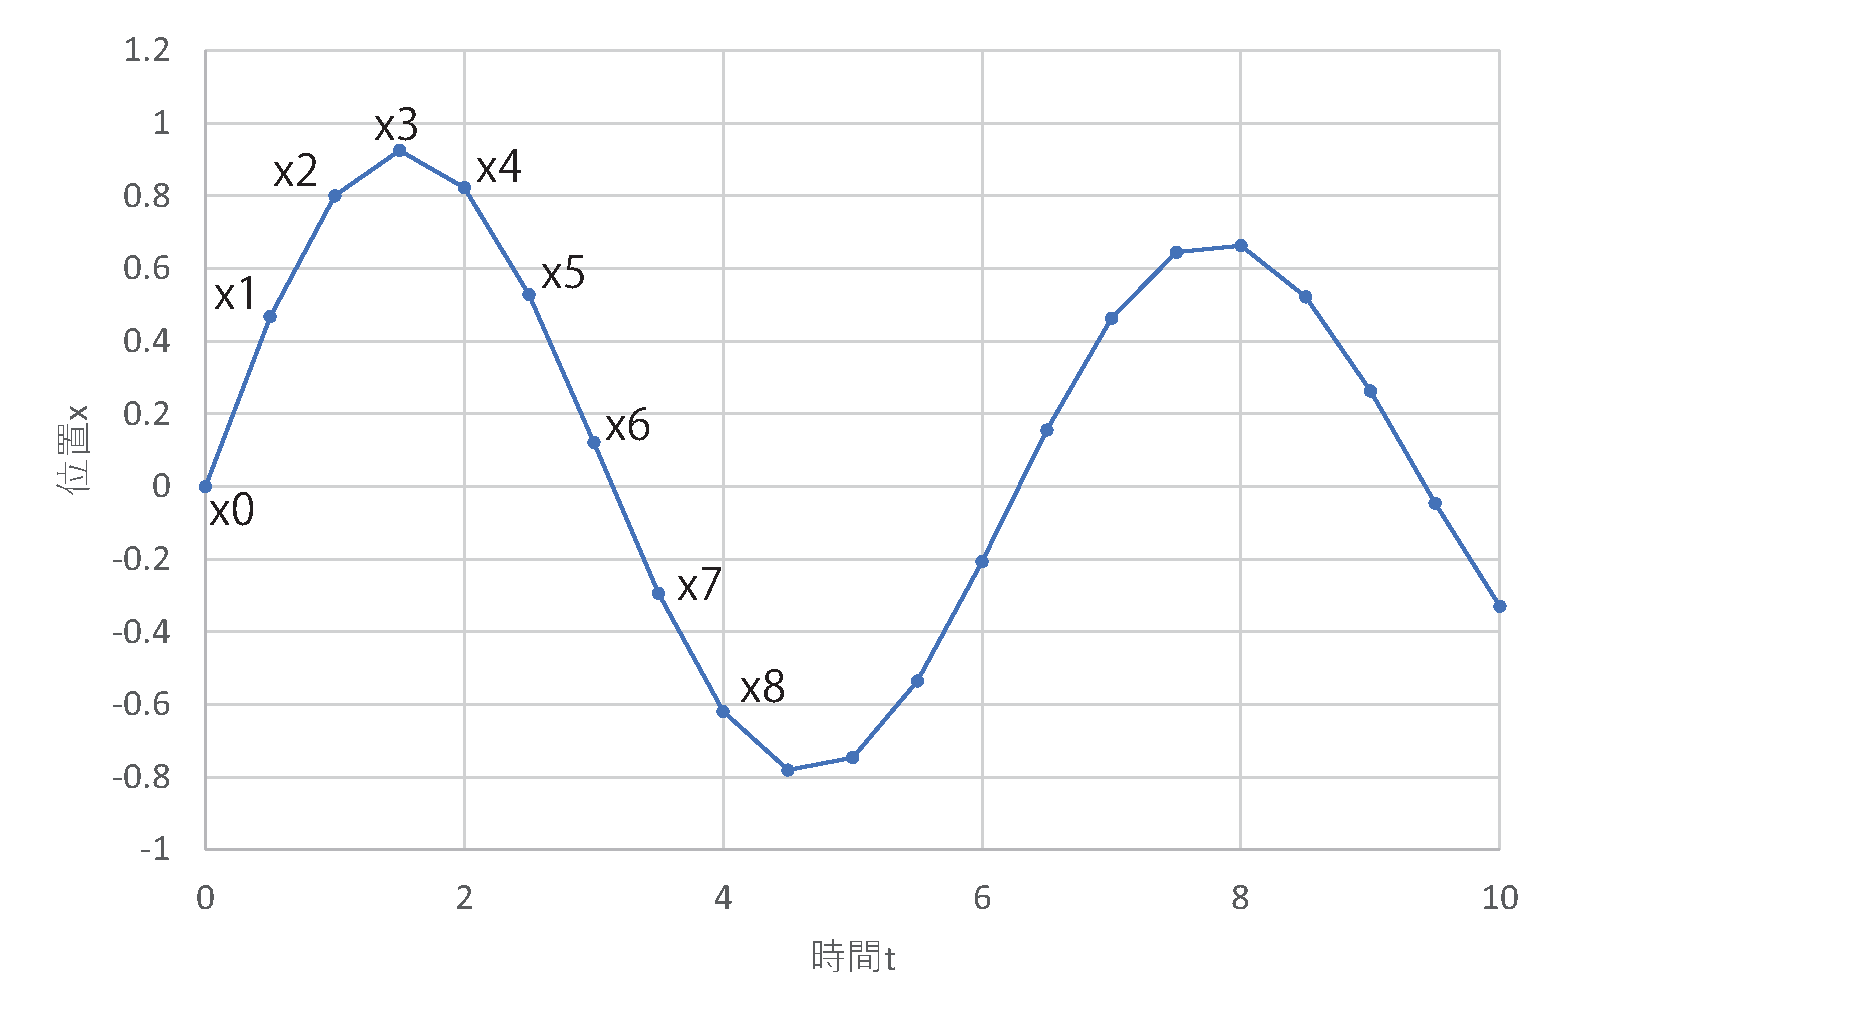
\includegraphics[width=\figSize\textwidth]{discrete.eps}
\caption{もともと時間的に滑らかに変化している変数をたくさんの離散値（折れ線）で近似する}
\label{fig:discrete}
\end{figure}
時間$i\Delta t$における微分を離散値で例えば次のように近似する。この近似は本授業で学ぶテーラー展開(Taylor expansion), マクローリン展開（Maclaurin expansion)を用いているが、やり方は今の段階で理解できなくてよい。ここで$v_i$は時刻iにおける速度（位置の一階微分）、$a_i$は時刻iにおける加速度（位置の二階微分）である。
\begin{eqnarray}
v_i &=& \frac{dx}{dt}_i \approx \frac{x_{i} - x_{i-1}}{\Delta t} \\
a_i &=& \frac{d^2 x}{dt^2}_i \approx \frac{x_{i} -2x_{i-1}+ x_{i-2}}{(\Delta t)^2} \label{eq:acc}
\end{eqnarray} 
Eq.~\ref{eq:acc}をEq.~\ref{eq:newton}に代入して、$F$が時間的に一定（たとえば重力$F=mg$, $g$は重力係数$9.8\mathrm{m^2/s}$）と考えると
\begin{equation}
m\frac{x_{i} -2x_{i-1}+ x_{i-2}}{(\Delta t)^2}   = F = mg
\end{equation}
となる。したがって過去の位置２つを使って未来の$x_i$を計算できる。つまり一般的には
\begin{equation}
x_i = g (\Delta t)^2 + 2x_{i-1} - x_{i-2}
\end{equation}
であり、書き下せば以下である。
\begin{eqnarray}
x_2 &=& g(\Delta t)^2 + 2x_1 - x_0 \\
x_3 &=& g(\Delta t)^2 + 2x_2 - x_1 \\
x_4 &=& g(\Delta t)^2 + 2x_3 - x_2 \label{eq:diff}\\
\vdots
\end{eqnarray}
重力加速度を$-9.8~\mathrm{m/s^2}$（マイナスは落下方向)、微小時間$\Delta t = 0.1 \mathrm{sec.}$、$x_o=x_1=0$で計算した値と、理論値$x=\frac{1}{2}g t^2$を比較するとFig.\ref{fig:drop}となり、よく近似できることが示されている。
\begin{figure}[hbt]
\centering
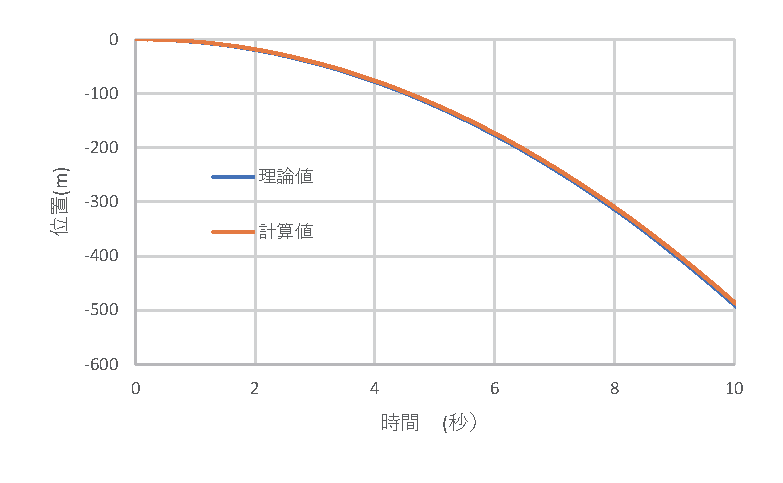
\includegraphics[width=\figSize\textwidth]{drop.eps}
\caption{差分方程式による自由落下シミュレーション}
\label{fig:drop}
\end{figure}
さらに、同じプログラム\footnote{実際はエクセル}に$x_o=0, x_1=4$の初期値を与えることで、投げ上げて自由落下する運動のシミュレーションやこの初速度で無重力($g=0$)のシミュレーションを行うこともできる(Fig.~\ref{fig:drops}, Fig.~\ref{fig:drop3}). 
\begin{figure}[hbt]
\centering
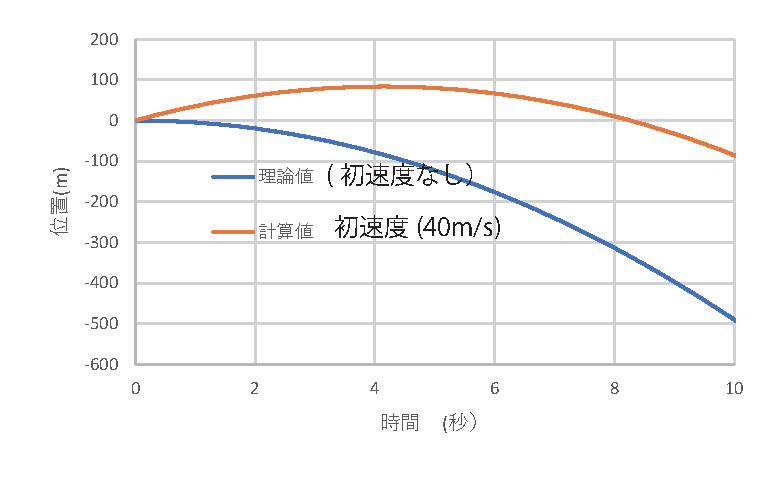
\includegraphics[width=\figSize\textwidth]{drops.eps}
\caption{差分方程式による初速度のある自由落下シミュレーション}
\label{fig:drops}
\end{figure}
\begin{figure}[hbt]
\centering
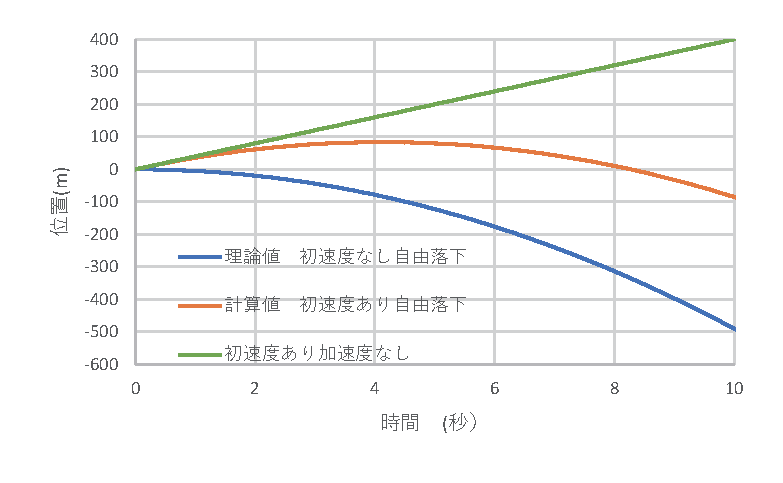
\includegraphics[width=\figSize\textwidth]{drop3.eps}
\caption{差分方程式による初速度ありで重力加速度がない場合のシミュレーション}
\label{fig:drop3}
\end{figure}
このように微分を微小時間に分割して近似する方法を差分方程式(difference equation)と呼ぶ。
\clearpage

%\section{積分}
%積分の勉強は、通常、与えられた関数(被積分関数:integrand)に対する積分を別の関数で表すことや、その積分値を求めることを学ぶ。例題として取り組むのは、面積や体積を求めることが典型的だが、現実には、面積や体積を関数の形で求めねばならないことはほとんどないし、面積や体積が求められるのは、地積や、地図などの複雑な形状である場合が多い。しかし積分が重要でない、ということではなく、積分は数値計算として実施されることや、さまざまな変換の中に組み込まれてしまっていることがほとんど、ということだ。
%
%先ほど取り組んだ微分方程式の解が実は積分に他ならないこと、時間で観測された信号を周波数という別の側面から観測するフーリエ変換（これも積分である）について説明する。
%
%%\subsection{微分方程式の解法}
%%微分と積分は逆の作用を及ぼす操作であり、先ほどの例で速度は位置の時間微分であることを述べたが、逆に速度から位置を求めるには、積分すればよい。以下にいくつか積分の例を示すが、どうやって結果が得られているか今わかる必要はない。
%%\begin{equation}
%%\int_{t=0}^t v dt  = \int_{t=0}^t \frac{dx}{dt} dt = x
%%\end{equation}
%%Fig.~\ref{fig:drop3}では加速度がなく初速度が与えられた場合のシミュレーション結果が示されているが、このように一定速度で移動するなら、位置は$vt$で求めることができる。つまり
%%\begin{equation}
%%\int_{t=0}^t v dt  = vt
%%\end{equation}
%%である。一方速度$v$は加速度を積分して得られるため、一定の重力加速度$g$が加わっている場合には
%%\begin{equation}
%%v = \int_{t=0}^t g dt = gt
%%\end{equation}
%%で与えられ、時間とともに一定の率で増加し、その積分として得られる位置$x$は
%%\begin{equation}
%%\int_{t=0}^t v dt = \int_{t=0} gt dt = \frac{1}{2}gt^2
%%\end{equation}
%%となる。これらの操作は、$g$が一定であることを使って積分記号$\int$の中の関数（被積分関数: integrand)が関数の形で積分している。$g$が時間に対して複雑に変化する場合には、関数の形で積分を求めることは多くの場合、難しい。
%%しかし差分方程式Eq.~\ref{eq:diff}の手順を使えば、$g$が時々刻々変わっても、位置$x$を計算することが可能である。
%%\vs
%%
%%差分方程式は、微分を離散値の組み合わせで表して、離散値に関する代数方程式を解くことで近似解を求める方法である。この他にも微分方程式をすべての時間で厳密に満足するのではなく、ある時間や領域の中で積分した状態で満足するように緩和させて近似解を求める重み付き残差法(Weighted residual method)が、電磁界解析や構造解析などで広く用いられている有限要素法解析(Finite Element Method)や、境界領域法(Boundary Element Method)の基本原理として用いられている。この方法を用いることで、微分方程式を連立方程式に変換して行列計算で解を求めることができる。
%%
%%少し式が複雑になるが例を示す。ニュートン運動方程式における$x$を既知の時間に関する関数$\Psi_o, \Psi_1, \cdots$ とそれらに対する重み関数$\bm{w}$をかけ合わせて、
%%\begin{equation}
%%x \approx \left[\begin{array}{ccc} \Psi_o & \Psi_1 & \cdots \end{array}\right] \left\{\begin{array}{c} w_o \\ w_1 \\ \vdots \end{array}\right\} = \bm{\Psi} \bm{w}
%%\end{equation}
%%と近似した場合、ニュートン運動方程式をうまく近似する重み係数$\bm{w}$を求めるため、損失関数$I(\bm{w})$を
%%\begin{equation}
%%I = \int (m\frac{d^2x}{dt^2} - F) x dt = \int \bm{w}^T \bm{\Psi}^T (m \frac{d^2\bm{\Psi}}{dt^2}\bm{w} - F) dt
%%\label{eq:wr}
%%\end{equation}
%%として、偏微分しそれが最大あるいは最小となるように$\bm{w}$を求める。このような手順で微分方程式をおおむね\footnote{おおむねというのは運動方程式が任意の時間で満足されている分けでなく、Eq.~\ref{eq:wr}の形式である範囲の中で平均的にという意図である}満足する近似解が$\bm{w}$に関する連立方程式を解くことで得られる。
%%\begin{eqnarray}
%%\frac{\partial I}{\partial \bm{w}} &=& \int m (\bm{\Psi}^T\frac{\partial^2 \Psi}{\partial t^2} + \frac{\partial^2 \Psi}{\partial t^2}^T\bm{\Psi})  \bm{w} - \bm{\Psi}^TF) dt \nonumber \\
%%&=& \int m (\bm{\Psi}^T\frac{\partial^2 \Psi}{\partial t^2} + \frac{\partial^2 \Psi}{\partial t^2}^T\bm{\Psi})dt  \bm{w} - \int \bm{\Psi}^TFdt = 0 
%%\end{eqnarray}
%
%\subsection{時間信号を周波数信号に変換する（フーリエ変換)}
%音は空気の疎密で伝達し、疎密が変わる速度が音の高さを表している。一秒間に疎密が変わる回数を周波数(frequency)とよび単位はHertz (Hz)である。音を数式で表すには、三角関数（サイン・コサイン）を用いる。周波数を$f$、時間を$t$、音の大きさを$A$としてサイン（余弦）を用いて、空気疎密の時間変化は
%\begin{equation}
%y = A\sin (2\pi f t ) 
%\label{eq:sound}
%\end{equation}
%と書ける。疎密の一周期は周期(period)と呼ばれる。440Hzの音による疎密の変化を図で書けばFig.~\ref{fig:f440}である。
%\begin{figure}[hbt]
%\centering
%\includegraphics[width=\figSize\textwidth]{f440.eps}
%\caption{440Hzの音の時間に応じた疎密の変化}
%\label{fig:f440}
%\end{figure}
%440 Hzの音の周期は1/440 = 0.00227 sec. = 2.27 msecである。本当は、空気の疎密は標準大気圧$p_o = 1013.25 \mathrm{hP_a} $ からのプラスマイナスで表されるため、圧力で表すと
%\begin{equation}
%y_p = A\sin(2\pi ft) + p_o
%\end{equation}
%であるが、音として認識されるのは振動している成分だけなので、Eq.~\ref{eq:sound}として問題ない。一オクターブ上の音は周波数が倍、一オクターブ下の音は周波数が半分であり、普通、ラ（A）の音は、27.5, 55, 110, 220, 440, 880, 1760, 3520 Hzとなる。オクターブ離れた音が同じ音として認識されるのは、低い音の周期に、高い音の周期が整数倍入ることと関係していると思うが、どうしてそのように知覚されるのかは、私にはわからない。440 Hzの音と880Hzの音の比較をFig.~\ref{fig:f440880}に示す。
%\begin{figure}[hbt]
%\centering
%\includegraphics[width=\figSize\textwidth]{f440880.eps}
%\caption{440Hzと880Hzの音の時間に応じた疎密の変化}
%\label{fig:f440880}
%\end{figure}
%
%一オクターブ離れた音の間には12の半音があり、それらの周波数は半音ごとに$\sqrt[\leftroot{10}12]{2}$(12回掛けると2になる数)倍づつ増えるように設定されている（平均律:equal temperament). A(440Hz)+C\#(554Hz)+E(659Hz)の和音を鳴らすと、それぞれのサイン波が足されて、Fig.~\ref{fig:atone}のような複雑な時間変化となる。
%\begin{figure}[hbt]
%\centering
%\includegraphics[width=\figSize\textwidth]{atone.eps}
%\caption{3つの音を同時に鳴らした場合の時間波形}
%\label{fig:atone}
%\end{figure}
%
%\vs
%上記では3つの音を足したが、異なる周期のサイン関数を掛け算すると、以下のように別の周波数$f_1+f_2$と$f_1-f_2$の音が発生する。導出には加法定理を用いたが、そこはわからなくてよい。重要なのは、2つの異なる周波数の音を掛けると、新な音が発生することであり、音であるからには、
%疎密（つまりマイナスとプラス）相互に発生するので、長期間時間積分するとゼロになるという点である。
%\begin{equation}
%y_1 y_2 = A_1 A_2 \sin(2\pi f_1t) \sin(2\pi f_2 t) = A_1 A_2 \frac{\cos(2\pi(f_1 + f_2)t) - \cos(2\pi(f1-f2)t)}{2}
%\end{equation}
%
%
%フーリエ変換（Fourier Transform）は、観測した時間波形$y(t)$から、積分を用いて含まれている周波数の分布$Y(f)$を特定する変換である（Fig.~\ref{fig:atonef})。
%\begin{figure}[hbt]
%\centering
%\includegraphics[width=\figSize\textwidth]{atonef.eps}
%\caption{フーリエ変換による時間波形から周波数分布への変換}
%\label{fig:atonef}
%\end{figure}
%Fig.~\ref{fig:atonef}は時間波形をフーリエ変換することで、3つの周波数(440, 554, 659)の存在を正確に特定している。
%
%
%フーリエ変換は、異なる周波数の信号を掛け合わせて作った信号は長期間積分するとゼロとなることを利用し、以下のように周波数信号を導く。この式は厳密ではないが、だいたいあってる。
%\begin{equation}
%Y(f) = \int_0^\infty y(t) \sin(2\pi ft) dt
%\label{eq:ft}
%\end{equation}
%$y(t)$は観測値として得られるが、Eq.~\ref{eq:ft}を積分して新たな関数を得ることは普通できない。そこで、式中の$\sin(2\pi ft)$部分を折れ線近似し、数値解析によってフーリエ変換を行う。
%この操作を離散フーリエ変換（Discrete Fourier Transform: DＦＴ）と呼ぶ。離散フーリエ変換にきわめて賢いアルゴリズムをあてはめ、精度を劣化させず高速計算を実現した手法が高速フーリエ変換(Fast Fourier Transform: FFT)である。
%
%
%時間波形を周波数波形に変換することは、周波数特定に留まらず、周波数の分布や特長を用いた話者特定や、音声認識にもつなげることができる。またWiFiやLTEでは、高速通信を安定的に行うために、デジタル信号を周波数変換してから送信する技術(OFDM/OFDMA: Orthogonal Frequency Division Multiplex/ Multiple Access)を採用しており、我々も実は日常的に用いている。

\bibliographystyle{unsrt}
\begin{thebibliography}{99}
\bibitem{tazawa}
 田澤義彦, ``しっかり学ぶ微分積分'', 東京電機大学出版局, (2008). 
\end{thebibliography}
\end{document}
 